\hebrewsection{Foundations of Digital Signal Processing}

\subsection{Introduction to Discrete-Time Signals}
A discrete-time signal $x[n]$ is a sequence of numbers, often derived from a continuous-time signal $x(t)$ through sampling. According to the \textbf{Nyquist-Shannon Sampling Theorem}, to reconstruct $x(t)$ perfectly, the sampling frequency $f_s$ must be greater than twice the maximum frequency $B$ present in the signal: $f_s > 2B$.

\subsubsection{Common Signal Sequences}
1. \textbf{Unit Impulse:} $\delta[n] = 1$ for $n=0$, else $0$.
2. \textbf{Unit Step:} $u[n] = 1$ for $n \geq 0$, else $0$.
3. \textbf{Exponential Sequences:} $x[n] = a^n u[n]$.

\subsection{Sampling and Aliasing}
When the Nyquist criterion is violated, high-frequency components are "folded" into lower frequencies, a phenomenon known as aliasing. This distortion is irreversible once the signal is sampled.

\subsection{Quantization and Coding}
Sampling discretizes time; quantization discretizes amplitude. A $B$-bit quantizer maps an infinite-precision sample to one of $2^B$ levels.
The \textbf{Signal-to-Quantization Noise Ratio (SQNR)} for a full-scale sinusoid is approximately:
\begin{equation}
    SQNR_{dB} \approx 6.02B + 1.76 \quad \text{dB}
\end{equation}
This "6 dB per bit" rule is a fundamental design constraint in ADC (Analog-to-Digital Converter) selection.

\subsection{Linear Time-Invariant (LTI) Systems}
An LTI system is characterized by:
\begin{enumerate}
    \item \textbf{Linearity:} $T\{a x_1[n] + b x_2[n]\} = a T\{x_1[n]\} + b T\{x_2[n]\}$.
    \item \textbf{Time-Invariance:} If $y[n] = T\{x[n]\}$, then $y[n-k] = T\{x[n-k]\}$.
\end{enumerate}

\subsubsection{The Convolution Sum}
The output of an LTI system is the convolution of the input $x[n]$ and the impulse response $h[n]$:
\begin{equation}
    y[n] = \sum_{k=-\infty}^{\infty} x[k]h[n-k]
\end{equation}

\subsection{Stability and Causality}
Stability in the BIBO (Bounded-Input Bounded-Output) sense is crucial. An LTI system is BIBO stable if $\sum |h[n]| < \infty$. Causality implies $h[n] = 0$ for $n < 0$.

\subsection{Difference Equations}
Discrete-time systems are often described by linear constant-coefficient difference equations:
\begin{equation}
    \sum_{k=0}^{N} a_k y[n-k] = \sum_{m=0}^{M} b_m x[n-m]
\end{equation}
The order of the system is $\max(N, M)$. This representation is the basis for practical implementations of IIR and FIR filters.

\subsection{The Z-Transform}
The Z-Transform $X(z)$ provides a frequency-domain-like representation for discrete signals:
\begin{equation}
    X(z) = \sum_{n=-\infty}^{\infty} x[n]z^{-n}
\end{equation}
The \textbf{Region of Convergence (ROC)} is the set of values in the complex plane for which the sum converges.

\subsubsection{Properties of the Z-Transform}
\begin{itemize}
    \item \textbf{Linearity:} $a x_1[n] + b x_2[n] \leftrightarrow a X_1(z) + b X_2(z)$.
    \item \textbf{Time Shifting:} $x[n-k] \leftrightarrow z^{-k} X(z)$.
    \item \textbf{Convolution:} $x[n] * h[n] \leftrightarrow X(z)H(z)$.
\end{itemize}

\subsection{Filter Structures}
Digital filters can be represented by difference equations. Porat (1997) identifies several key structures:
\begin{itemize}
    \item \textbf{Direct Form I:} Straightforward implementation of the difference equation.
    \item \textbf{Direct Form II (Canonic):} Uses the minimum number of delay elements by sharing them between the feedback and feedforward paths.
    \item \textbf{Cascade and Parallel Forms:} Used to reduce sensitivity to coefficient quantization by breaking high-order systems into 2nd-order sections (SOS).
\end{itemize}

\subsection{Group Delay and Phase Analysis}
Group delay $\tau_g(\omega)$ is the negative derivative of the phase. It represents the time delay of the signal's envelope at a specific frequency. Nonlinear phase (varying group delay) causes dispersion, where different frequency components travel at different speeds.

\begin{center}
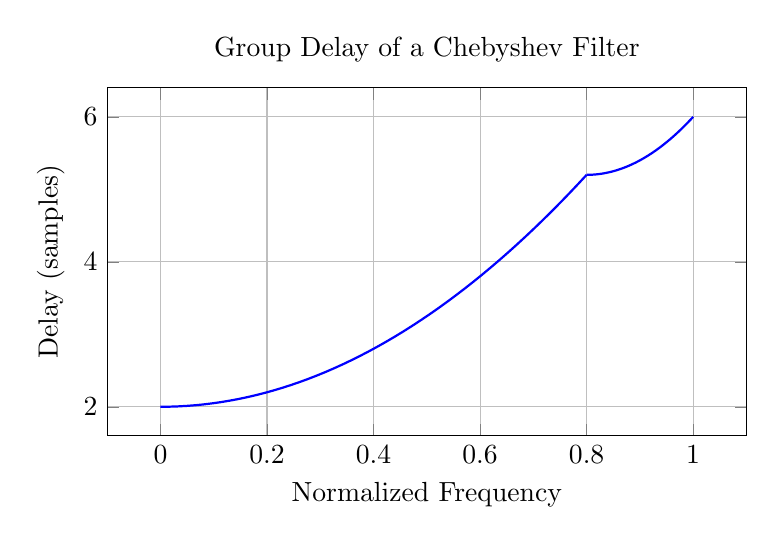
\begin{tikzpicture}
\begin{axis}[
    title={Group Delay of a Chebyshev Filter},
    xlabel={Normalized Frequency},
    ylabel={Delay (samples)},
    grid=major,
    width=0.8\textwidth,
    height=6cm
]
\addplot[blue, thick, domain=0:0.8, samples=50] {2 + 5*x^2};
\addplot[blue, thick, domain=0.8:1, samples=50] {5.2 + 20*(x-0.8)^2};
\end{axis}
\end{tikzpicture}
\end{center}

\subsection{The Hilbert Transform}
The Hilbert transform is used to create the \textbf{analytic signal}, which has no negative frequency components. This is essential for SSB modulation and complex envelope representation.
\begin{equation}
    \hat{x}[n] = x[n] * \frac{1}{\pi n}
\end{equation}
In the frequency domain, it corresponds to a -90 degree phase shift for positive frequencies.

\subsection{Multi-rate Signal Processing}
Multi-rate systems use different sampling rates at various stages of processing. This is fundamental in modern transceivers for decimation (reducing $f_s$) and interpolation (increasing $f_s$).

\subsubsection{Decimation and Aliasing}
To reduce the sampling rate by an integer factor $M$, we must first apply a low-pass \textbf{anti-aliasing filter} with cutoff $\pi/M$. Then, we keep only every $M$-th sample:
\begin{equation}
    y[n] = x[nM]
\end{equation}

\subsubsection{Interpolation and Imaging}
To increase the sampling rate by a factor $L$, we insert $L-1$ zeros between samples and then apply an \textbf{anti-imaging low-pass filter} with cutoff $\pi/L$.

\subsection{Sampling of Bandpass Signals}
The Nyquist theorem for bandpass signals with bandwidth $B$ centered at $f_c$ allows sampling at rates much lower than $2f_c$, specifically $2B < f_s < 2B(1 + 1/n)$ for some integer $n$, provided aliasing does not overlap the signal spectra.
